\chapter{Data} \label{cha:data}

In this chapter, we survey the available datasets and examine how their characteristics may influence our models.
For our work to be of any practical use, it is imperative that we collect data that is as diverse as possible, representing a wide range of imaging conditions and patient backgrounds.
While large datasets for image-level graded images are available, the lesion segmentation task suffers from a severe lack of pixel-wise segmented data, and even fewer provide both grading and semantic label information.

In the field of data science, fully understanding the properties of your data domain is just as imperative as model development.
Exploratory data analysis provides the necessary context and insights to choose the appropriate modelling techniques and put forth an informed interpretation of one's results.

\section{FGADR}

\begin{figure}[h]
    \centering
    \begin{subfigure}{0.45\textwidth}
        \centering
        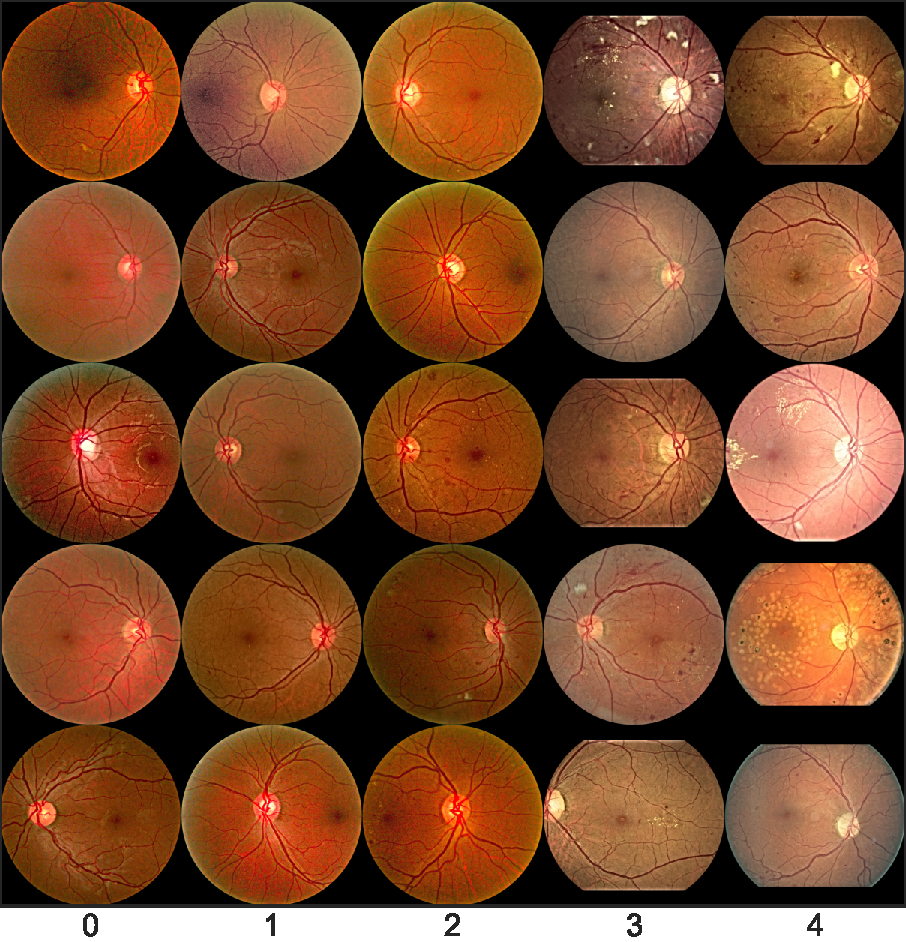
\includegraphics[width=\linewidth]{datasets/figs/fgadr_real_sample.pdf}
        \caption{Retinal fundus images.}
        \label{fig:fgadr_sample_real}
    \end{subfigure} %
    \begin{subfigure}{0.45\textwidth}
        \centering
        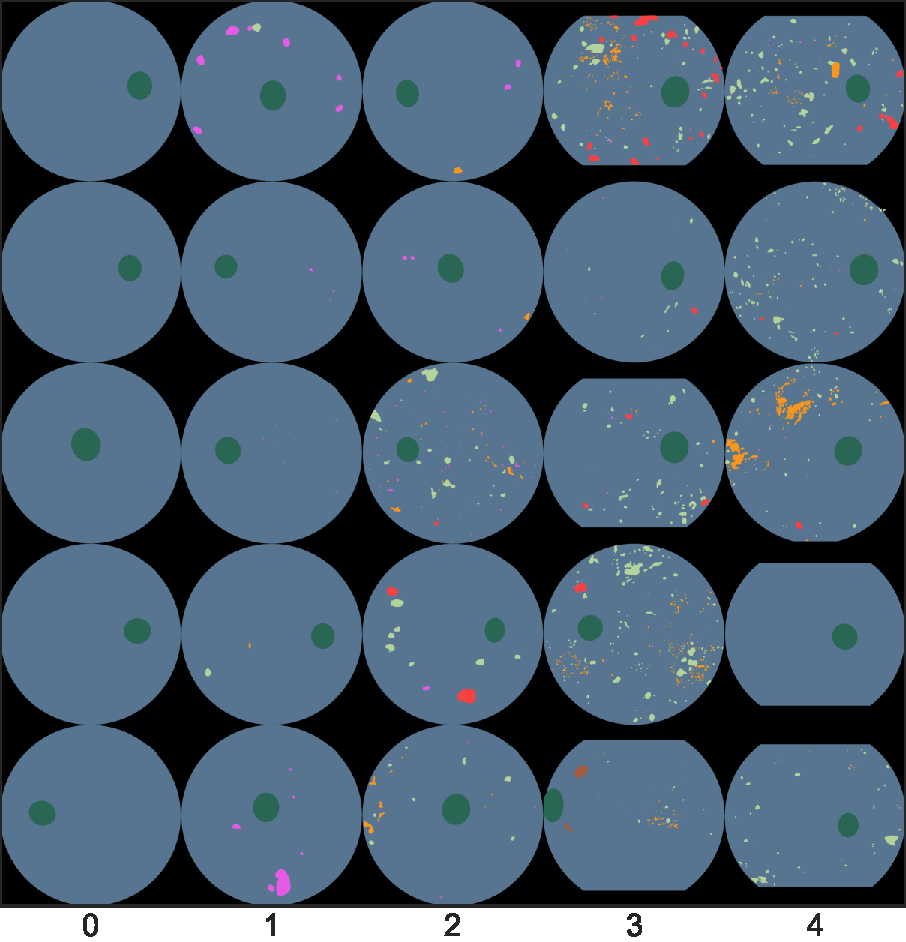
\includegraphics[width=\linewidth]{datasets/figs/fgadr_label_sample.pdf}
        \caption{Corresponding semantic labels.}
        \label{fig:fgadr_sample_label}
    \end{subfigure}
        \caption{A sample of images from the FGADR dataset and accompanying manual semantic annotations. Columns from left to right correspond to DR grades 0 through 4.}
    \label{fig:fgadr_sample}
\end{figure}

The Fine-Grained Annotated Diabetic Retinopathy (FGADR) dataset \cite{Zhou2020b} was released in 2020 alongside DR-GAN, and consists of two subsets.
The first, called the \emph{Seg-set}, contains 1842 images with both image-level annotations for DR severity, and pixel-level annotations for microaneurysms, haemorrhages, hard exudates, soft exudates, intraretinal microvascular abnormalities, and neovascularization.
Optic disc masks are not provided, so manual annotations were collected for this project (provided in \Cref{sec:od}).
The second, called the \emph{Grade-set}, contains 1000 images with only image-level DR grades.
It is useful for its high annotation confidence, however the \emph{Grade-set} is still pending approval by the researcher's legal department at the time of writing, and therefore is regrettably not available for use in this project.
All images in both sets have a resolution of $1280 \times 1280$.
This is the only pixel-wise annotated dataset that includes labels for neovascularization and intraretinal microvascular abnormalities, which is of particular significant since according to \Cref{tab:dr_stages}, NV and IRMA are key to differentiating stage 3 from stage 4.

\Cref{fig:fgadr_sample} shows a sample of images and associated annotations from the FGADR dataset.
Visually, the relationship between the prevalence of lesions and DR grade is clear.
Note that overlap of semantic labels is possible with the images.
We resolve these arbitrarily, based on the index of the label (according to \Cref{tab:mappings}).
The photographs themselves are noisier than those from the other datasets, which can likely be attributed to the illumination conditions at the time of imaging.

% \begin{figure}[h]
%     \centering
%         \centering
%         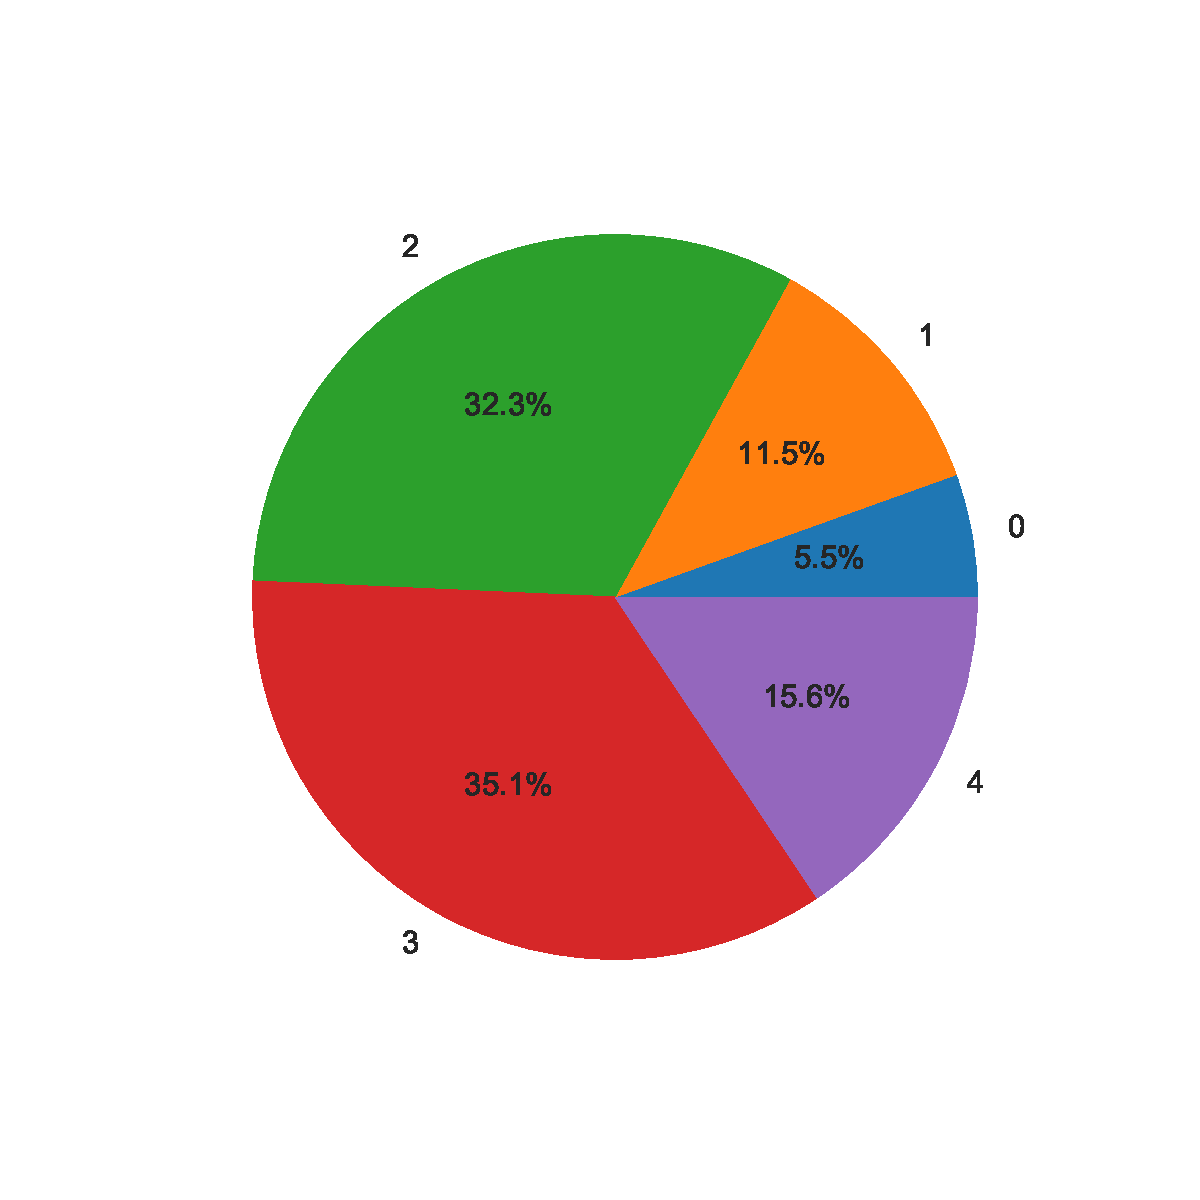
\includegraphics[width=0.5\textwidth]{datasets/figs/fgadr_grade_dist.pdf}
%         \label{fig:fgadr_seg_grade_dist}
%     \caption{Distribution of DR grades in the FGADR \emph{Seg-set}.}
%     \label{fig:fgadr_grade_dist}
% \end{figure}
% 
% \Cref{fig:fgadr_grade_dist} shows the distribution of DR grades in the dataset.
% Grades 0 and 1 are underrepresented in the \emph{Seg-set} as a side-effect of the dataset creation process.

\begin{figure}[h]
    \centering
    \begin{subfigure}{0.45\textwidth}
        \centering
        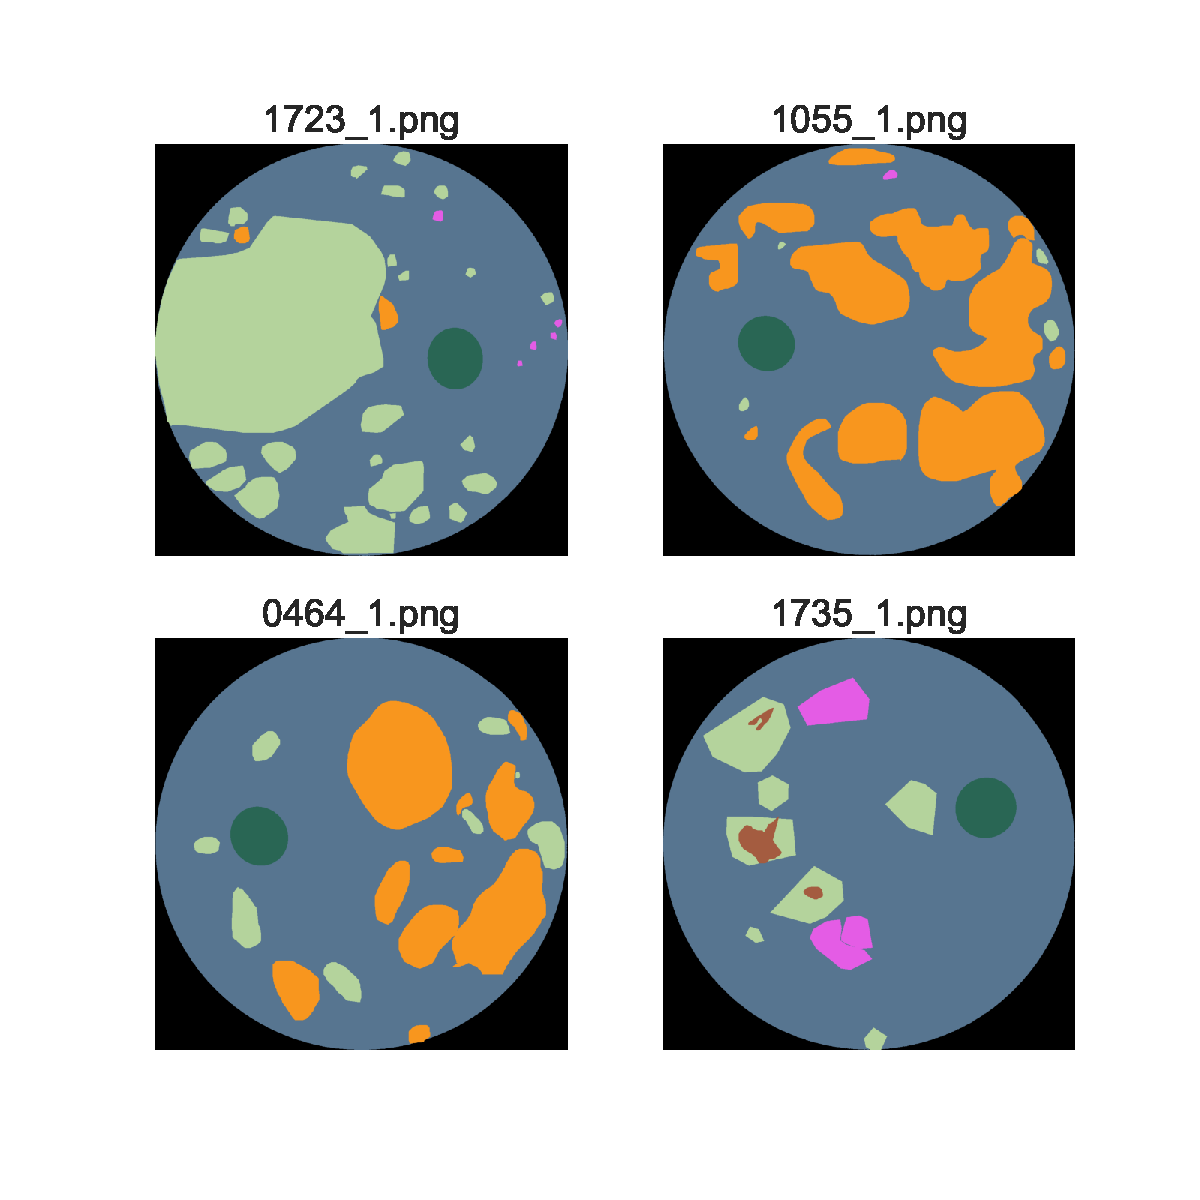
\includegraphics[width=\linewidth]{datasets/figs/fgadr_bad_sample.pdf}
        \caption{Sample of images from batch 1.}
        \label{fig:fgadr_bad_sample}
    \end{subfigure} %
    \begin{subfigure}{0.45\textwidth}
        \centering
        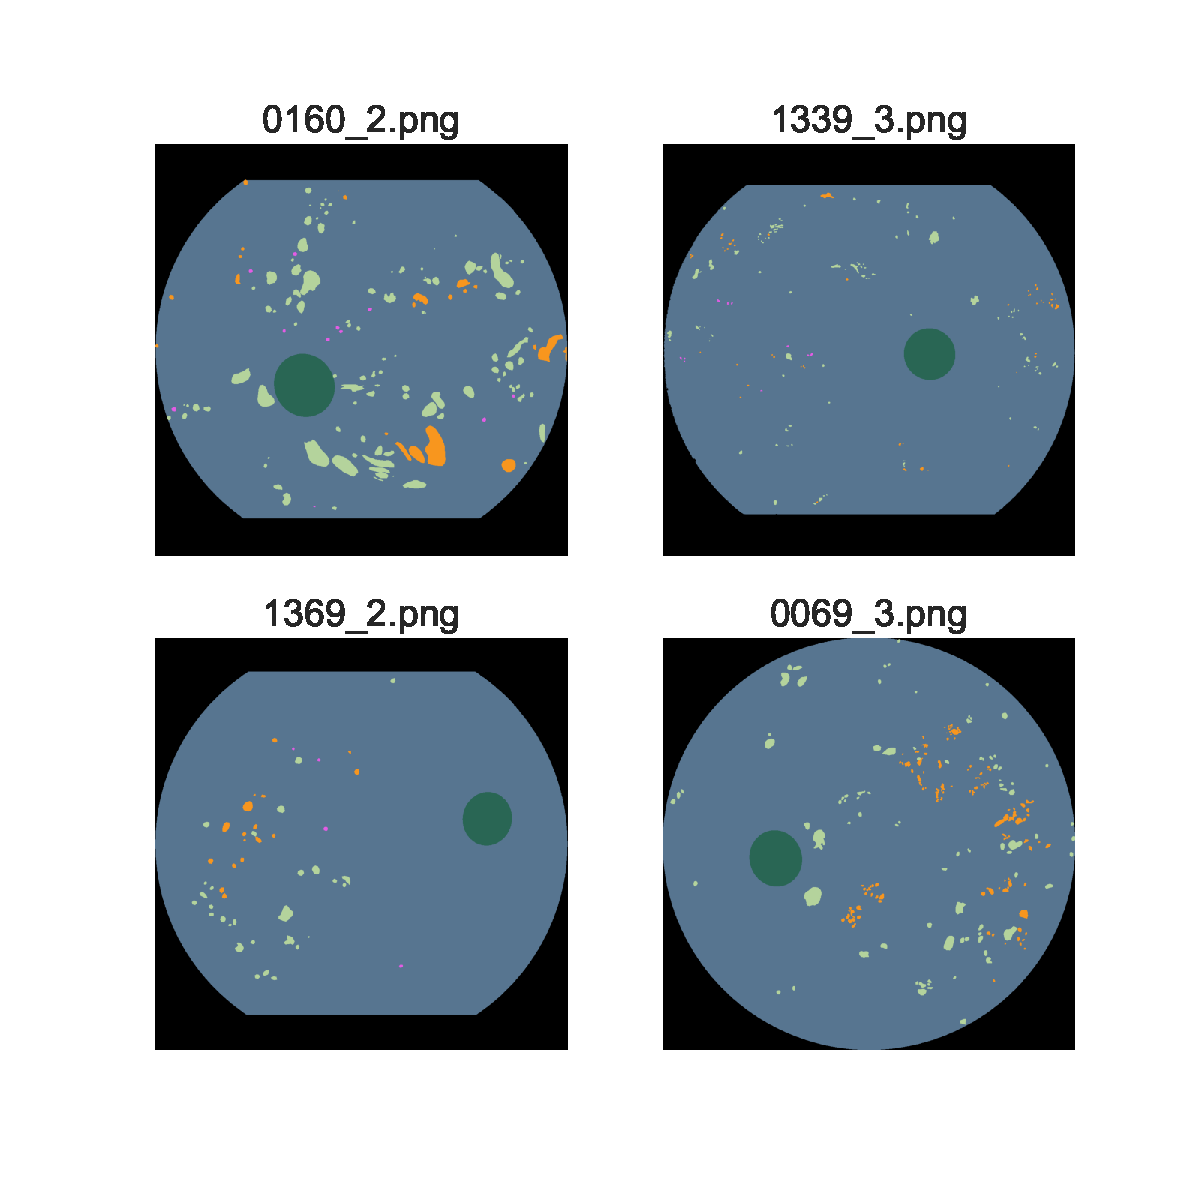
\includegraphics[width=\linewidth]{datasets/figs/fgadr_good_sample.pdf}
        \caption{Sample of images from batches 2 and 3.}
        \label{fig:fgadr_good_sample}
    \end{subfigure}
    \caption{Comparison of annotator bias between batches.}
    \label{fig:fgadr_good_bad}
\end{figure}

Interestingly, a visual examination of the annotations reveals a number of samples which are incongruously annotated compared to the other samples, likely due to annotator bias.
These coarsely annotated files all share a file suffix, following the pattern \lstinline{XXXX_1.png}, a selection of these are shown in \Cref{fig:fgadr_good_bad}.
While not entirely clear from the dataset's descriptor paper, this may indicate the grader, hospital, or something else.
This suffix value can be one of \lstinline{1}, \lstinline{2}, or \lstinline{3}, and we'll refer to this number as the ``batch''.
Apart from the style of annotation, another difference is that this group of files do not have the top and bottom section of the retina cropped, while the other groups have a mix.
One way of removing this bias would be to exclude all 1000 images which contain this suffix. 
However, this is not viable for three reasons: first, this batch makes up over half of the dataset so we would be drastically limiting the amount of available data; secondly, not all of these images suffer from coarse annotations; and finally, this batch represents the entirety of images with grades 0, 1, and 2, removing them would heavily imbalance our data.
Instead, we manually review each of the images in this batch and list those that are determined to be ``too coarse'' (by a non-expert and subjective measure).
We call this the ``FGADR exclusion list'', and can be found in \Cref{sec:fgadr_excl}.

\begin{figure}[h]
    \centering
    \begin{subfigure}{0.45\textwidth}
        \centering
        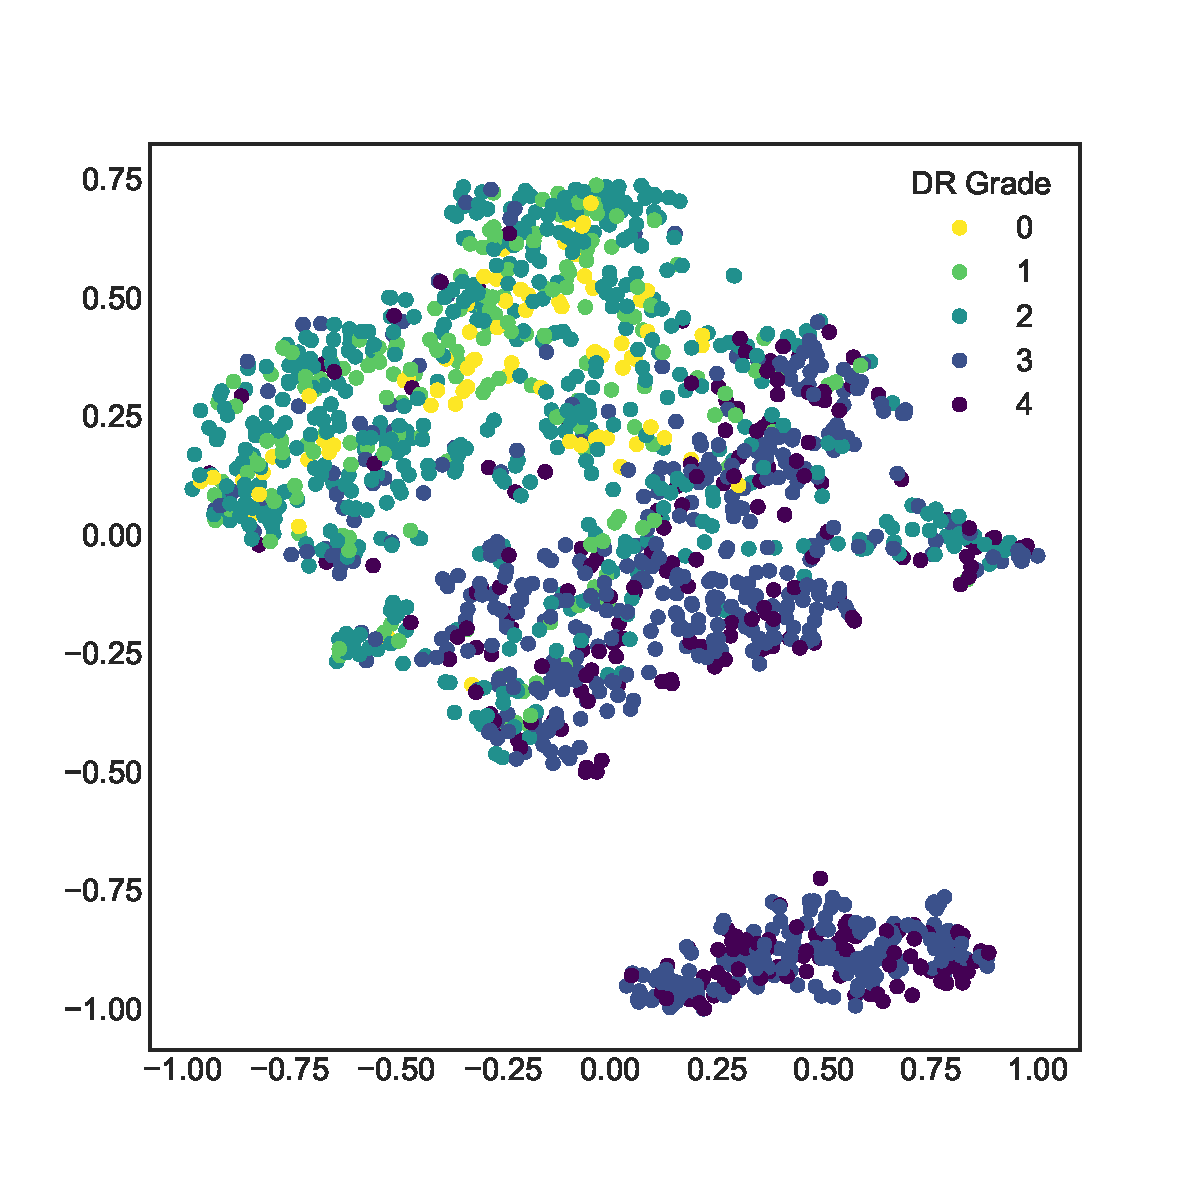
\includegraphics[width=\linewidth]{datasets/figs/fgadr_label_tsne.pdf}
        \caption{Coloured by DR severity grade.}
        \label{fig:fgadr_tsne_grade}
    \end{subfigure} %
    \begin{subfigure}{0.45\textwidth}
        \centering
        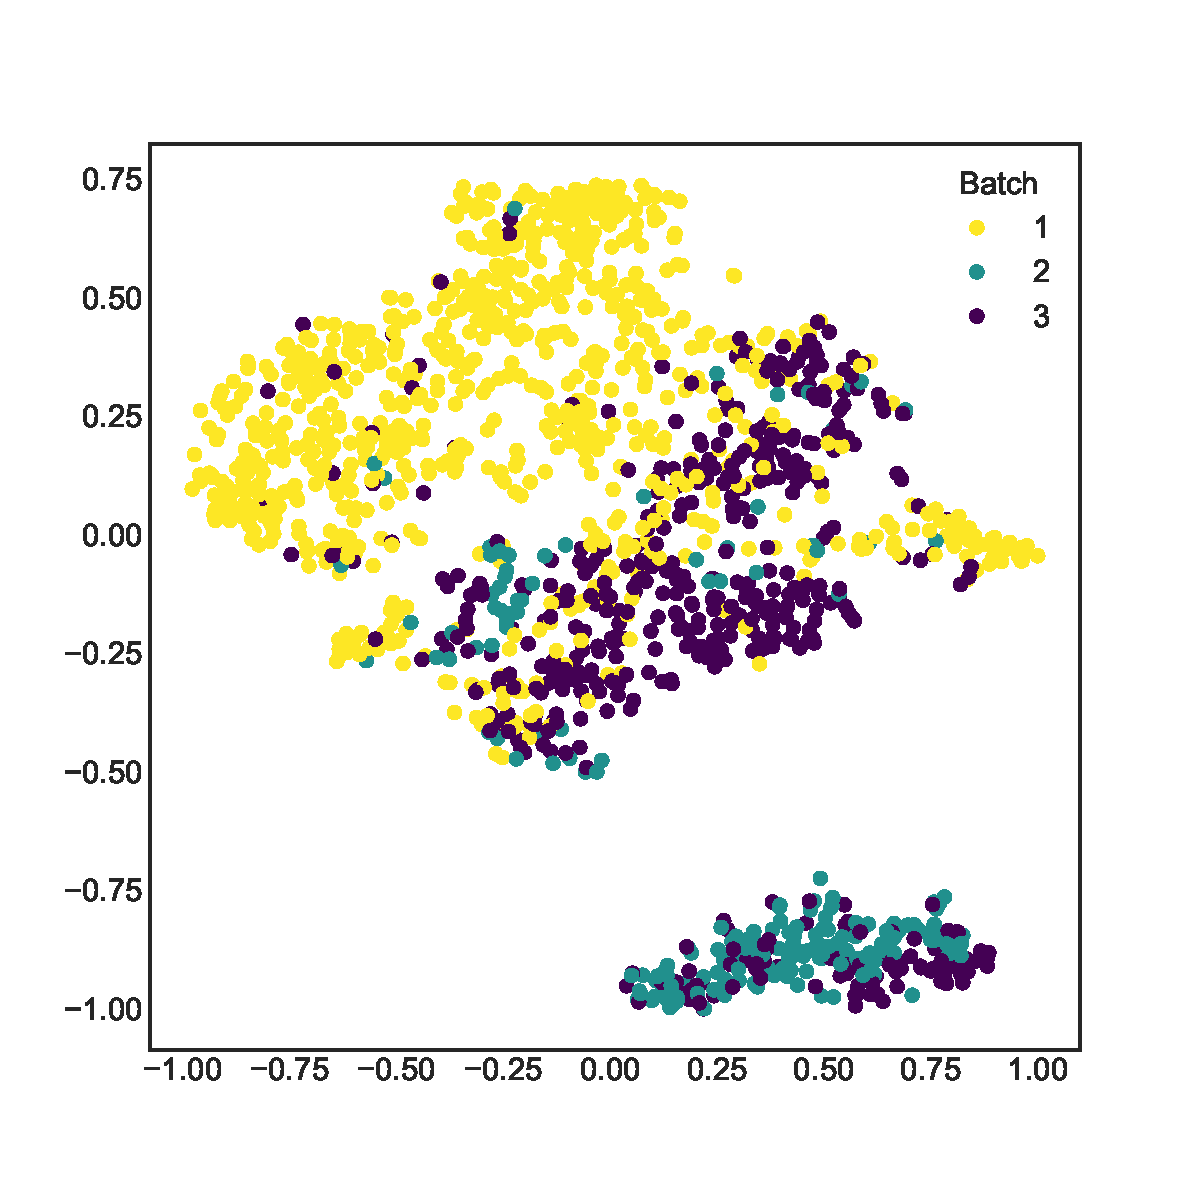
\includegraphics[width=\linewidth]{datasets/figs/fgadr_batch_tsne.pdf}
        \caption{Coloured by batch number.}
        \label{fig:fgadr_tnse_grader}
    \end{subfigure}
    \caption{t-SNE applied to feature vectors extracted from ResNet-50 trained on FGADR labels.}
    \label{fig:fgadr_tsne}
\end{figure}

To deepen our understanding the relationships present in the data, we can apply a dimensionality reduction technique such as t-SNE to create a visual representation which may reveal underlying patterns.
We use the ResNet-50 network as a feature extractor by training it to predict the DR grade of semantic labels from the FGADR dataset.
Note that, while pre-trained networks (on datasets like ImageNet) are commonly used for feature extraction, we decided to train from scratch since our data domain bears little resemblance to those used to train general-purpose networks.
Once trained, we can then extract the learned feature vectors from the layer immediately prior to the final fully-connected layer.
During training, the network was able achieve to 0.86 accuracy on the training set, and 0.53 accuracy on the validation set, which is an indication that there is at least some predictive power in the images.
This relationship is confirmed visually by examining the result of running t-SNE on these feature vectors, shown in \Cref{fig:fgadr_tsne_grade}.
There is a distinct separation between images which have a high DR severity and low DR severity, even if the clusters are not particularly well-defined.

However, given the discrepancy between image batches we identified earlier, it's possible that the features being calculated are more to do with the batch.
To explore this possibility, we plot the same t-SNE components, but this time colour the points by the batch number, depicted in \Cref{fig:fgadr_tnse_grader}.
There are two factors at play here: difference in features between batches, and grade distribution.
For instance, as mentioned earlier, all images with grade 0, 1, and 2 belong to batch 1, and this is reflected in the dimensionality reduction.
The isolated cluster in the lower-right corner is an example of the latter factor, and consists of images which have the top and bottom sections cropped.
While interesting, we expect that there is sufficient diversity within the dataset, and the final training dataset will further combine multiple other datasets, and hence does not pose an obstacle.

\section{IDRiD}

\begin{figure}[h]
    \centering
    \begin{subfigure}{0.45\textwidth}
        \centering
        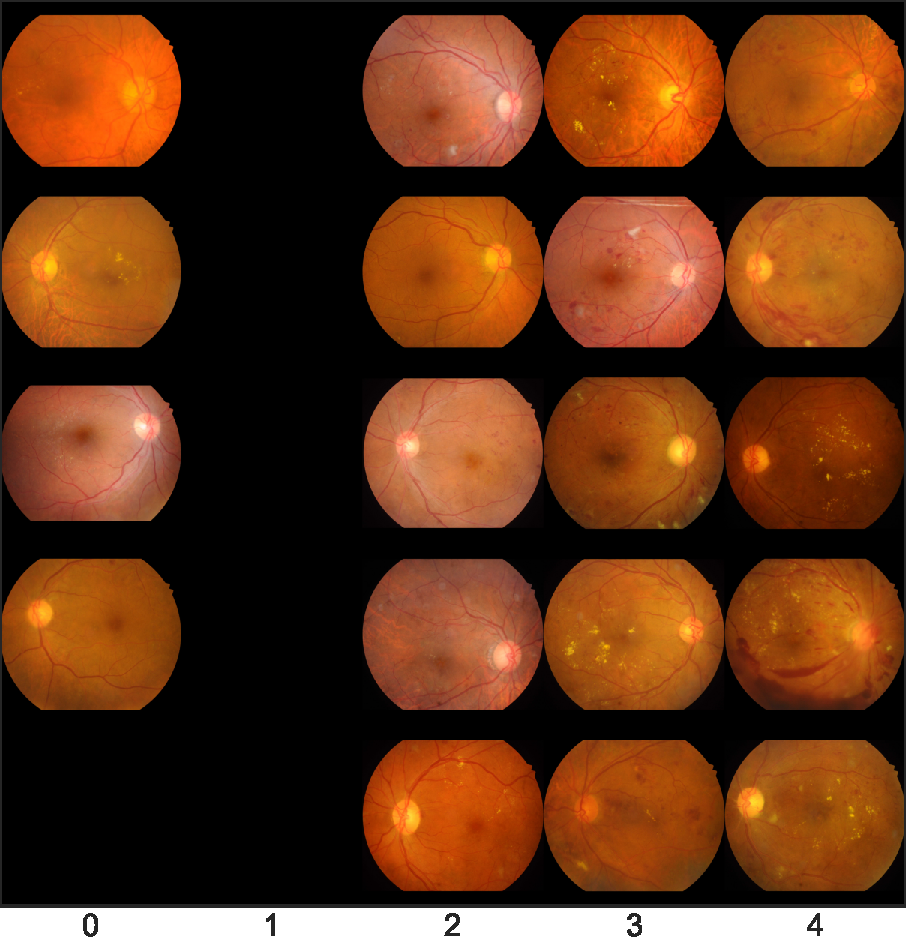
\includegraphics[width=\textwidth]{datasets/figs/idrid_real_sample.pdf}
        \caption{Retina fundus images.}
        \label{fig:idrid_sample_real}
    \end{subfigure} %
    \begin{subfigure}{0.45\textwidth}
        \centering
        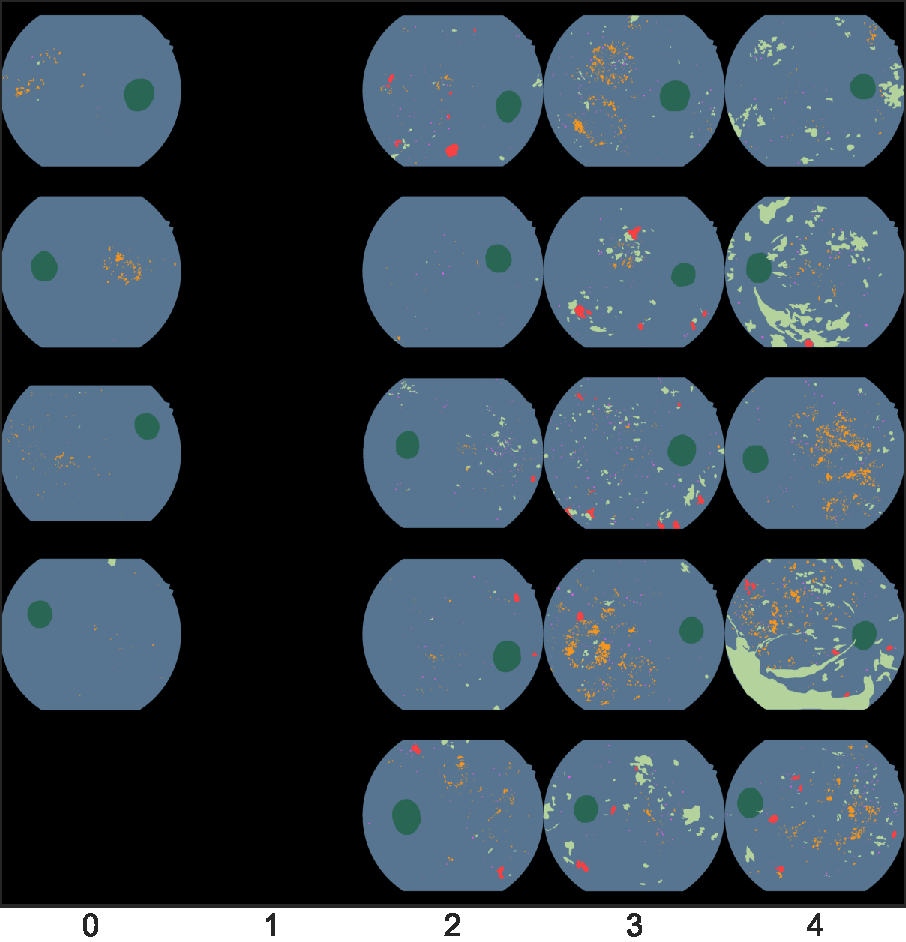
\includegraphics[width=\textwidth]{datasets/figs/idrid_label_sample.pdf}
        \caption{Corresponding semantic labels.}
        \label{fig:idrid_sample_label}
    \end{subfigure}
        \caption{A sample of images from the IDRiD dataset and accompanying manual semantic annotations. Columns from left to right correspond to \emph{inferred} DR grades 0 through 4.}
    \label{fig:idrid_sample}
\end{figure}

The Indian Diabetic Retinopathy Image Dataset (IDRiD) \cite{Porwal2018} was initially released in 2018 as part of the ``Diabetic Retinopathy: Segmentation and Grading Challenge'' held at ISBI-2018.
Similarly to the FGADR dataset, the IDRiD dataset also consists of multiple subsets.
The first subset, aimed at training segmentation models, contains 81 retinal fundus images with varying levels of DR, each of which are accompanied by pixel-level annotations for the optic disc, microaneurysms, soft exudates, hard exudates, and haemorrhages.
Unlike FGADR, annotations for neovascularization, intraretinal microvascular abnormalities, or image-level DR grades for these images are not provided.
The second subset, aimed at training classification models, consists of 516 images annotated with DR severity grades only.
The images in the second subset are exclusive with those in the first subset, and thus none of the images in this dataset contain both image-level and pixel-level annotations, as in the FGADR dataset.
Each image has a resolution of $4288\times 2848$.

To obtain inferred DR grades on this dataset for weakly-supervised learning, we train a model to predict the DR grade from the retinal fundus images.
This method is given in greater detail in \Cref{sec:grade_inference}.
The distribution of the resulting grades has relatively few grade 0s since all images exhibit some form of DR.
There are no grade 1 images, which can likely be attributed tsto bias in the grade inference network.

\section{E-Ophtha}

\begin{figure}[h]
    \centering
    \begin{subfigure}{0.45\textwidth}
        \centering
        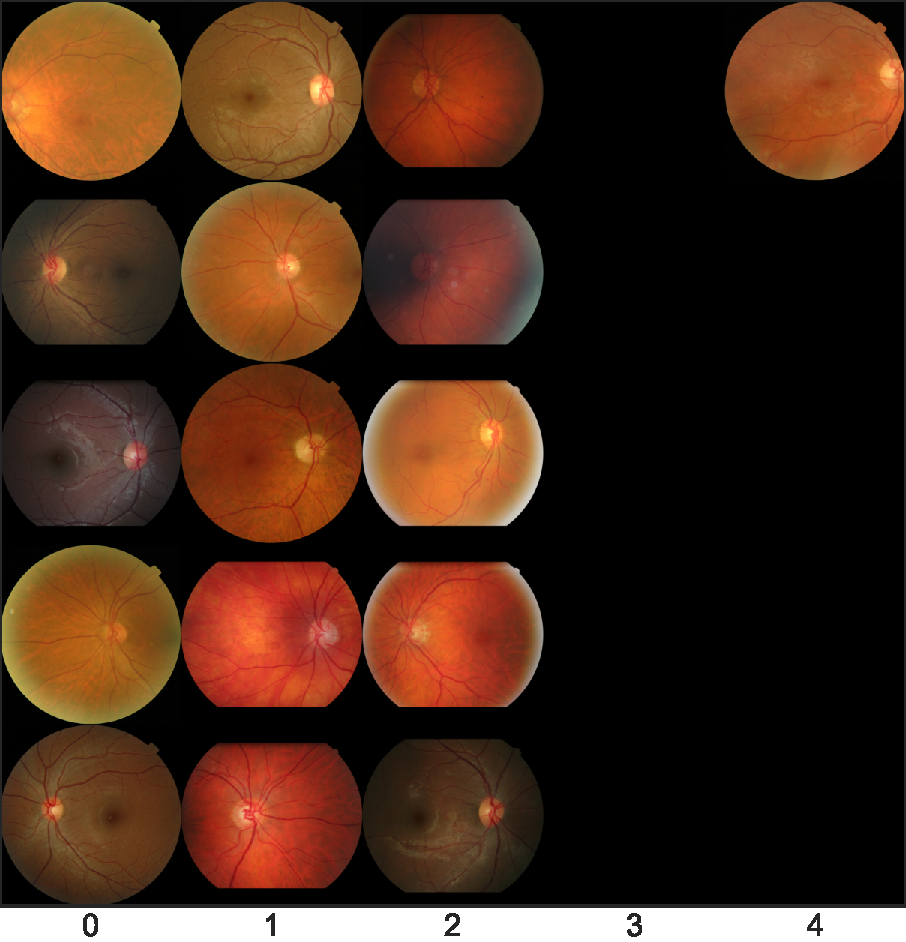
\includegraphics[width=\textwidth]{datasets/figs/eophtha_real_sample.pdf}
        \caption{Retina fundus images.}
        \label{fig:eophtha_sample_real}
    \end{subfigure} %
    \begin{subfigure}{0.45\textwidth}
        \centering
        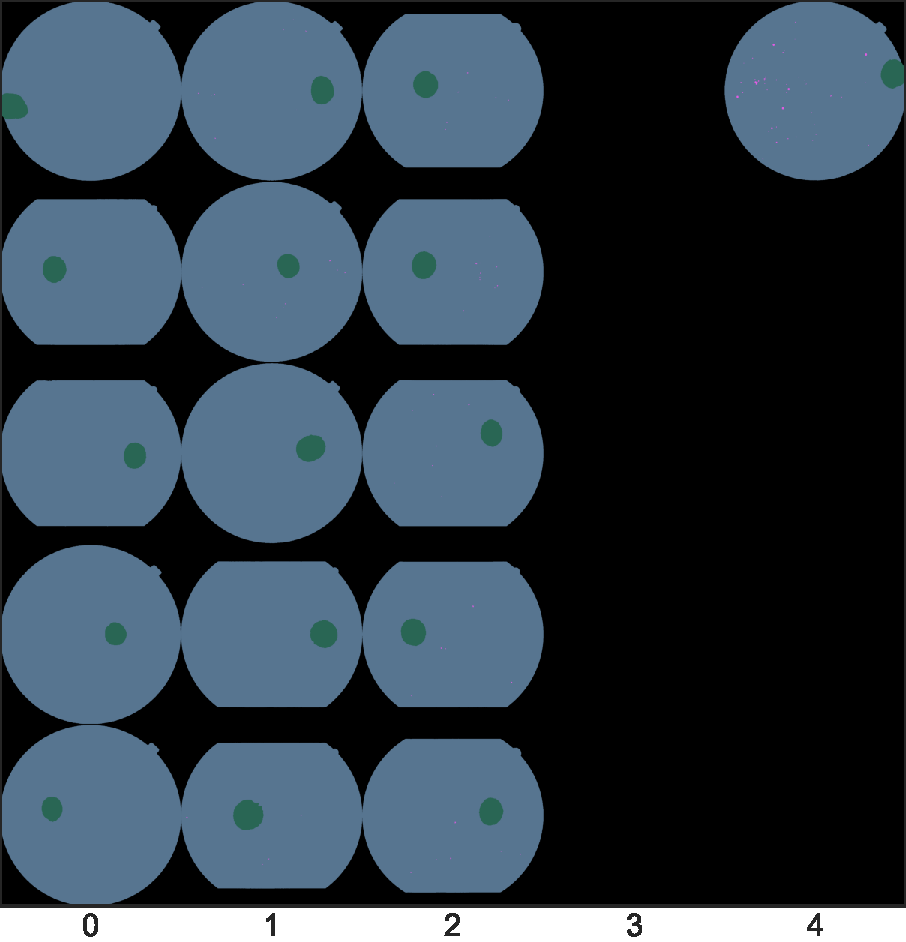
\includegraphics[width=\textwidth]{datasets/figs/eophtha_label_sample.pdf}
        \caption{Corresponding semantic labels.}
        \label{fig:eophtha_sample_label}
    \end{subfigure}
        \caption{A sample of images from the e-ophtha dataset and accompanying manual semantic annotations. Columns from left to right correspond to \emph{inferred} DR grades 0 through 4.}
    \label{fig:eophtha_sample}
\end{figure}

The e-ophtha\footnote{Sometimes (mis-)spelled ``e-optha'' in the dataset files.} \cite{eoptha} dataset was released in 2013 and contains pixel-level annotations for exudates (it is not specified whether these are hard or soft exudates) and microaneurysms.
The images are provided as two subsets: e-ophtha-EX and e-ophtha-MA, each of which also contains a number of ``healthy'' images which do not exhibit the respective lesion (but may have other lesions).
In total, 26 images are annotated with exudates only, 128 are annotated with microaneurysms only, 21 are annotated with both, and 269 images are not annotated with any kind of lesion.
Image resolution varies from $1440 \times 960$ to $2544 \times 1696$.
A sample of images is shown in \Cref{fig:eophtha_sample}; notice how the density of annotations here is much less than those in the FGADR and IDRiD datasets.
This can be largely attributed to the fact that fewer lesion types are annotated, as well as the annotations simply being more fine-grained.
For this dataset, instead of manually annotating optics discs, we infer them using a model as described in \Cref{sec:optic_disc_inference}.

\section{EyePACS}

The EyePACS dataset was first released in 2015 for the Kaggle Diabetic Retinopathy Detection challenge \cite{eyepacs}. 
It is the largest dataset of retinal fundus images for the purpose of grading the severity of diabetic retinopathy, consisting of 88,702 images graded from 0 to 4.
Pixel-level annotations are not provided.
Despite the large volume of data, the quality of images is highly variable, particularly compared to the other datasets we are using, which appear to be more closely curated.
Moreover, the labels are highly imbalanced, with 73.5\% of images being grade 0, and just 2.0\% being grade 4.
For the purpose of the original competition, public/private training and testing sets are provided, but we disregard these and instead create our own subsets.

\section{Data Split}

\begin{figure}[h]
    \centering
    \begin{subfigure}{0.3\textwidth}
        \centering
        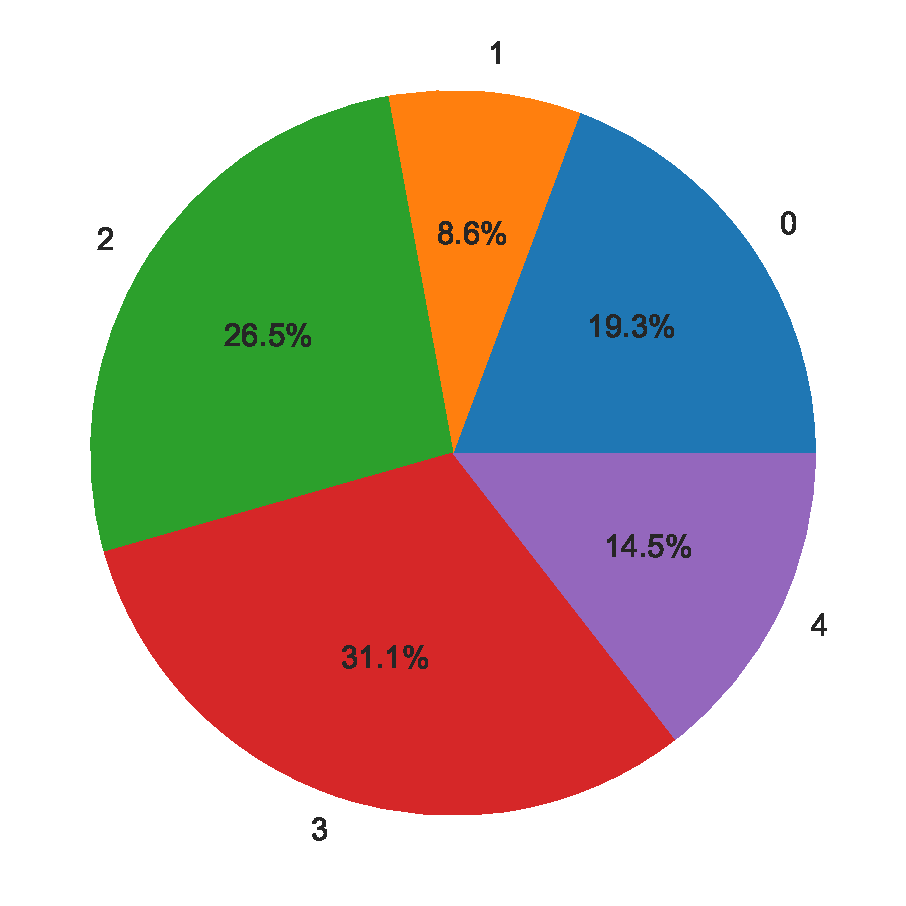
\includegraphics[width=\textwidth]{datasets/figs/combined_grade_dist.pdf}
        \caption{Segmentation dataset.}
        \label{fig:segmentation_grade_dist}
    \end{subfigure}
    \begin{subfigure}{0.3\textwidth}
        \centering
        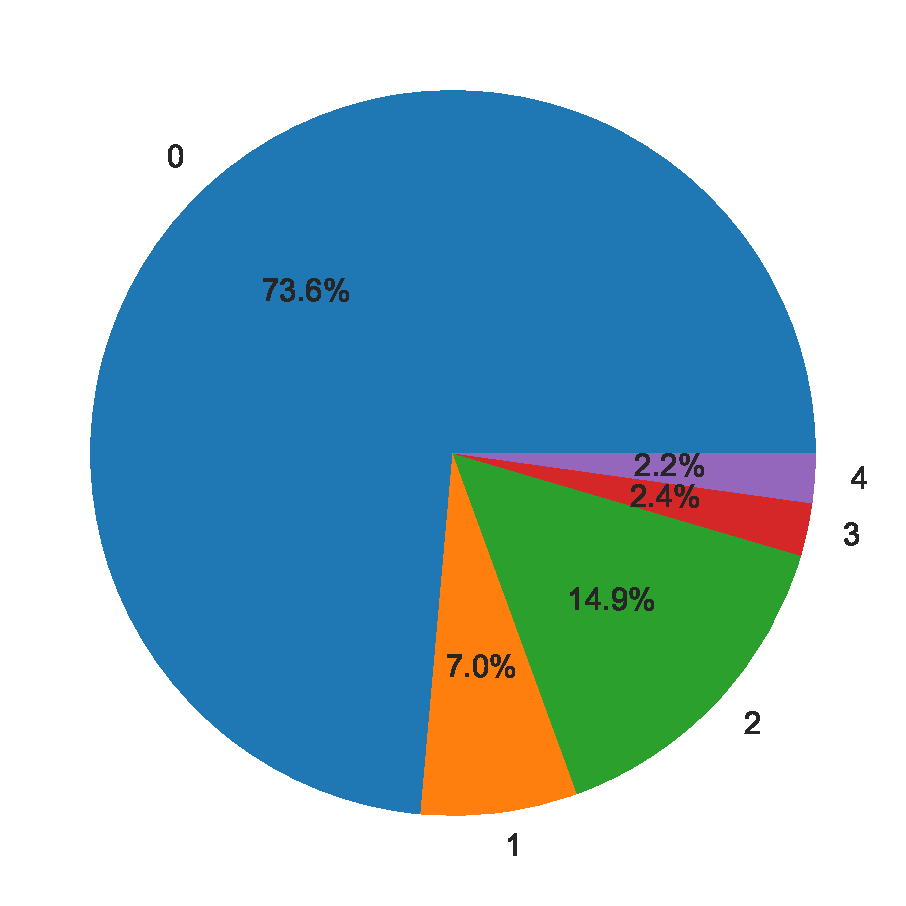
\includegraphics[width=\textwidth]{datasets/figs/eyepacs_grade_dist.pdf}
        \caption{EyePACS dataset.}
        \label{fig:eyepacs_grade_dist}
    \end{subfigure}
    \begin{subfigure}{0.3\textwidth}
        \centering
        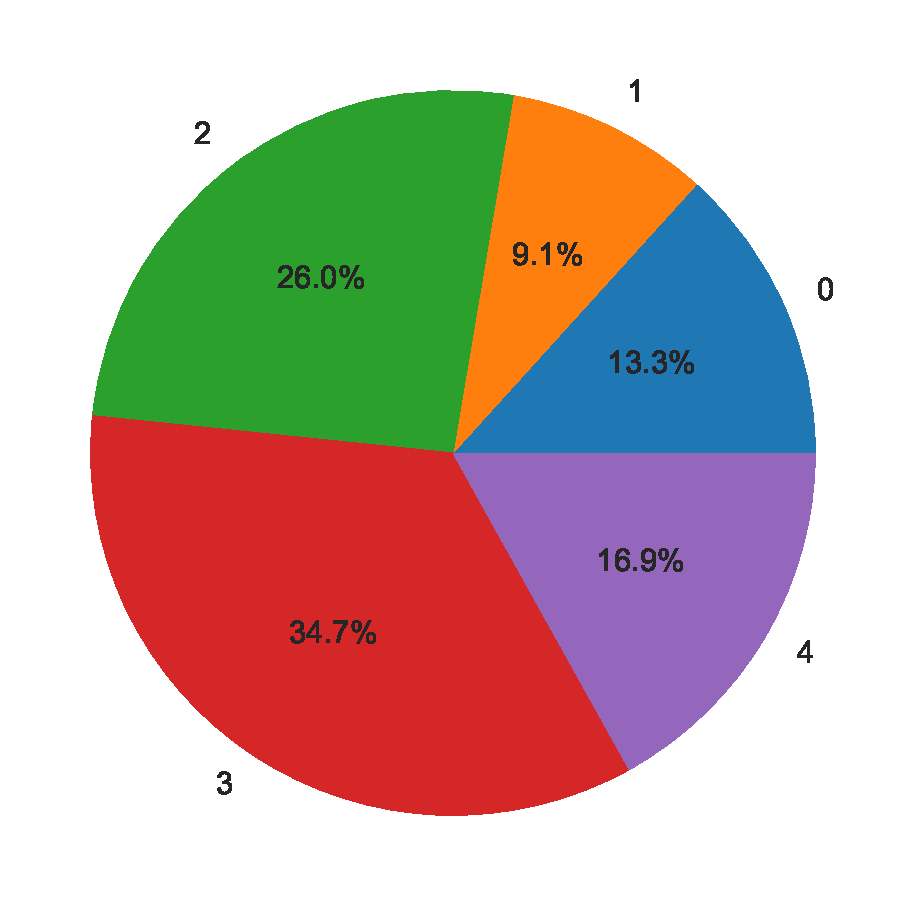
\includegraphics[width=\textwidth]{datasets/figs/grading_grade_dist.pdf}
        \caption{Grading dataset.}
        \label{fig:grading_grade_dist}
    \end{subfigure}
    \caption{Distribution of DR grades in various datasets.}
    \label{fig:combined_grade_dist}
\end{figure}

We combine the FGADR, IDRiD, and e-ophtha datasets to train our semantic label generation models.
In order to prevent data leakage, we randomly separate out (and fix) training, validation, and test sets, according to \Cref{tab:label_split}.
We train all generative models on the training set, compare models using the validation set, and use the test set for the final evaluation.

\begin{table}[h]
    \centering
    \begin{tabular}{lrrrrr}
        \toprule
        \multirow{2}{*}{Subset} & \multirow{2}{*}{Proportion} & \multicolumn{4}{c}{\# Images} \\
        \cmidrule{3-6}
         & & FGADR & IDRiD & e-ophtha & Total \\
        \midrule
        Training & 0.80 & 1194 & 61 & 352 & 1607 \\
        Validation & 0.10 & 151 & 13 & 37 & 201 \\
        Test & 0.10 & 149 & 7 & 45 & 201 \\
        \midrule
        Total & 1.00 & 1494 & 81 & 434 & 2009 \\
        \bottomrule
    \end{tabular}
    \caption{Data split for segmentation data.}
    \label{tab:label_split}
\end{table}

For the EyePACS training set we simply take a training and test split, according to \Cref{tab:eyepacs_split}.

\begin{table}[h]
    \centering
    \begin{tabular}{lrr}
        \toprule
        Subset & Proportion & \# Images \\
        \midrule
        Training & 0.80 & 70,961 \\
        Test & 0.20 & 17,741 \\
        \midrule
        Total & 1.00 & 88,702 \\
        \bottomrule
    \end{tabular}
    \caption{Data split for the EyePACS dataset.}
    \label{tab:eyepacs_split}
\end{table}

We also create a small grading set by combining samples from FGADR \emph{Seg-set} and the IDRiD grading set, shown in \Cref{tab:grading_split}.
We use the same FGADR training set from the segmentation split to avoid data leakage.
This is not a concern for the IDRiD dataset since the IDRiD segmentation and grading datasets are mutually exclusive.

\begin{table}[h]
    \centering
    \begin{tabular}{lrrrr}
        \toprule
        \multirow{2}{*}{Subset} & \multirow{2}{*}{Proportion} & \multicolumn{3}{c}{\# Images} \\
        \cmidrule{3-5}
         & & FGADR & IDRiD & Total \\
        \midrule
        Training & 0.80 & 1194 & 412 & 1606 \\
        Validation & 0.10 & 151 & 52 & 203 \\
        Test & 0.10 & 149 & 52 & 201  \\
        \midrule
        Total & 1.00 & 1494 & 516 & 2010  \\
        \bottomrule
    \end{tabular}
    \caption{Data split for grading data.}
    \label{tab:grading_split}
\end{table}

\section{Other Datasets}

Other datasets for diabetic retinopathy related tasks are available, but were inappropriate for our use case.
Specific reasons are given below:
\begin{description}
    \item[DiaRetDB0] \hfill \\ Released in 2006 as part of the ImageRet\footnote{\url{https://www.it.lut.fi/project/imageret}} project.
    DiaRetDB0 does not have pixel-level annotations, only image-level annotations labelling the presence of lesions.
    DiaRetDB1 and DiaRetDB1 v2 were also released by the ImageRet project.
    \item[DiaRetDB1] \hfill \\ Contains 89 images at a resolution of $1500\times 1152$, 84 of which show signs of DR and five which are healthy.
    Images are accompanied by pixel-wise labels for hard exudates, soft exudates, microaneurysms, and ``red small dots'' -- which we interpret as haemorrhages. 
    Labels are not provided for neovascularization or intraretinal microvascular abnormalities, nor are image-level DR grades.
    Interestingly, each image was annotated independently by four different experts, and a confidence level was provided for each marking.
    Unfortunately, after running some experiments, we determined that the annotations are too coarse to be used as segmentation maps.
    However, we still collected manual optic disc annotations for these images, also provided in \Cref{sec:od}.
    \item[DiaRetDB1 v2] \hfill \\ Contains the same data as DiaRetDB1 but in a more flexible data format.
    \item[DRIVE] \hfill \\ Contains 40 images with pixel-level segmentations for vessels only.
    \item[CHASE\_DB1] \hfill \\ Contains 28 images with pixel-level segmentations for vessels only.
    \item[STARE] \hfill \\ Contains 400 images with pixel-level segmentations for vessels only.
    \item[DRISHTI-GS] \hfill \\ Contains 101 images with pixel-level segmentations for the optic disc only.
    \item[Messidor] \hfill \\ Contains 1200 images graded by their risk of diabetic macular oedema, instead of diabetic retinopathy.
\end{description}

\section{Data Pre-Processing}

\begin{figure}[h]
    \centering
    \begin{subfigure}{0.45\textwidth}
        \centering
        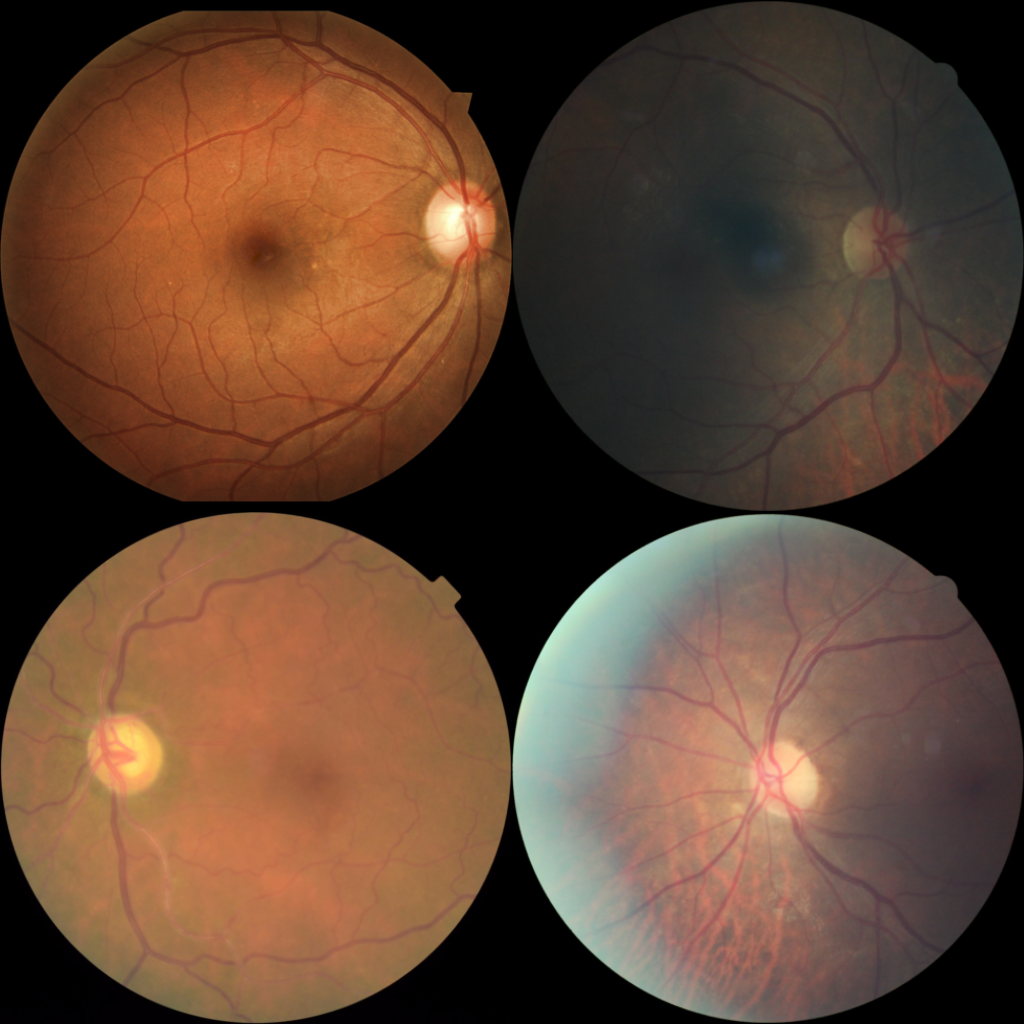
\includegraphics[width=\linewidth]{datasets/figs/eyepacs_before.png}
    \end{subfigure} %
    \begin{subfigure}{0.45\textwidth}
        \centering
        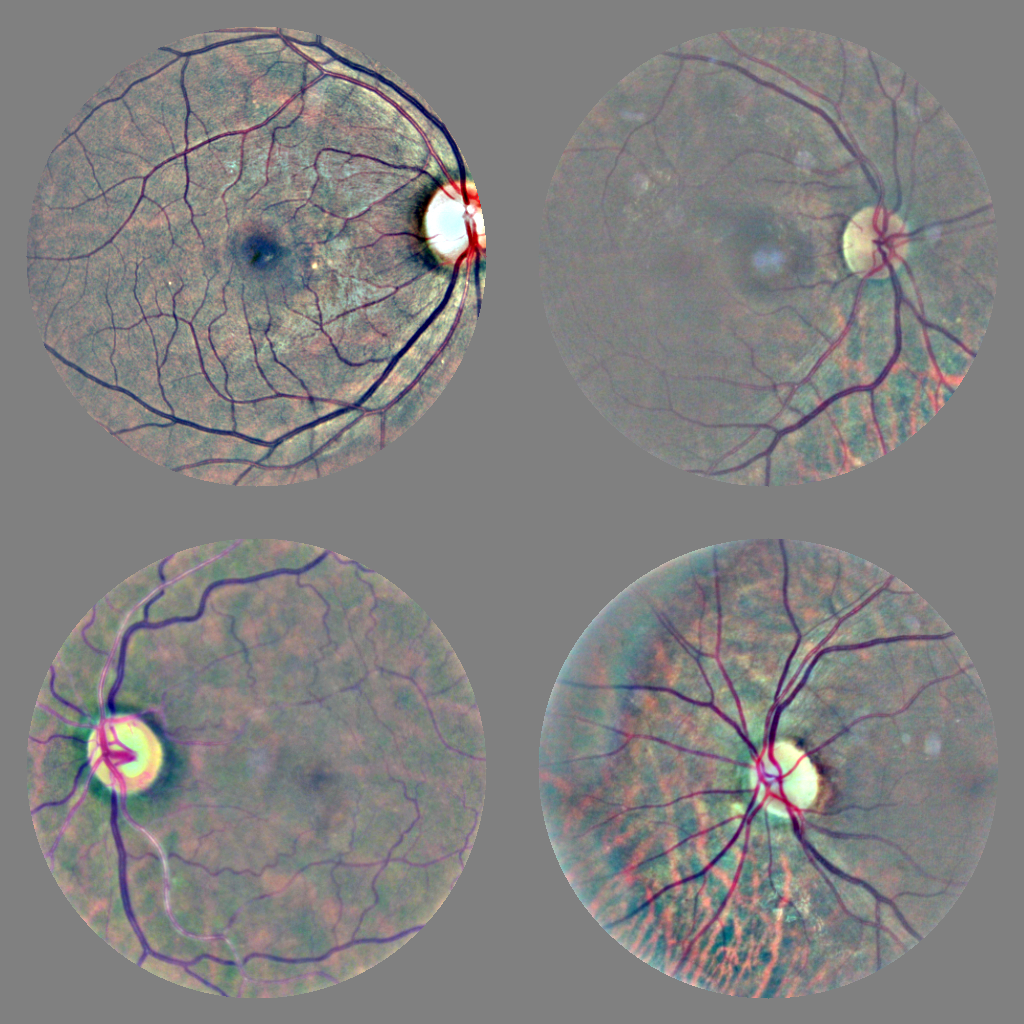
\includegraphics[width=\linewidth]{datasets/figs/eyepacs_after.png}
    \end{subfigure}
    \caption{Before (left) and after (right) illumination correction.}
    \label{fig:preprocess_before_after}
\end{figure}
To ensure image size and retina positioning is uniform across all images, we perform the following steps:
\begin{enumerate}
    \item Extract a mask for the retinal fundus boundary by performing a binary threshold.
    \item Draw a bounding box around this boundary.
    \item Crop around the bounding box so that the retina is now centred and fills the image.
    \item Pad to square.
    \item Resize to $1280 \times 1280$.
\end{enumerate}
To further correct for illumination differences between retina photographs, we borrow image processing techniques from Benjamin Graham \cite{benjamingraham}, winner of the 2015 Kaggle Diabetic Retinopathy Challenge\footnote{\url{ https://www.kaggle.com/c/diabetic-retinopathy-detection}}:
\begin{enumerate}
    \setcounter{enumi}{5}
    \item Subtract the local average.
    \item Clip the radius to remove boundary effects.
\end{enumerate}
Each pixel-annotated dataset provides binary masks for each lesion class.
The segmentation masks for each class are combined into a single-channel image, where the discrete value of each pixel encodes its label.
That is, each retina semantic label with height $H$ and width $W$ is represented as an image $M \in \mathbb{L}^{H\times W}$ where $\mathbb{L} = \{ 0, 1, 2, 3, 4, 5, 6, 7, 8 \}$, ensuring that every pixel belongs to exactly one class.
For clarity, the semantic labels have been mapped to RGB colours according to \Cref{tab:mappings}.

\newcommand{\thiscolor}[1]{\hfill \texttt{\convertcolorspec{named}{#1}{RGB}\RGBcolor (\RGBcolor)} \fcolorbox{black}{#1}{\hspace{2mm}}}

\definecolor{retina}{RGB}{87, 117, 144}
\definecolor{od}{RGB}{41, 102, 84}
\definecolor{ma}{RGB}{228, 92, 229}
\definecolor{he}{RGB}{180, 211, 156}
\definecolor{ex}{RGB}{248, 150, 30}
\definecolor{se}{RGB}{249, 65, 68}
\definecolor{nv}{RGB}{250, 208, 44}
\definecolor{irma}{RGB}{164, 92, 64}
\definecolor{bg}{RGB}{0, 0, 0}

\begin{table}[h]
    \centering
    \begin{tabular}{lcr}
    \toprule
        Label & Value & RGB Colour \\
    \midrule
        Retina & 0 & \thiscolor{retina}\\ 
        Optic Disc & 1 & \thiscolor{od}\\ 
        Microaneurysms & 2 & \thiscolor{ma} \\ 
        Haemorrhages & 3 & \thiscolor{he} \\ 
        Hard Exudates & 4 & \thiscolor{ex} \\ 
        Soft Exudates & 5 & \thiscolor{se} \\ 
        Neovascularization & 6 & \thiscolor{nv} \\ 
        Intraretinal Microvascular Abnormalities & 7 & \thiscolor{irma} \\ 
        Background & 8 & \thiscolor{bg} \\ 
    \bottomrule
    \end{tabular}
    \caption{Semantic label values and colour mappings.}
    \label{tab:mappings}
\end{table}

\section{Grade Inference} \label{sec:grade_inference}

To infer grades, a ResNet-101 network was trained for 20 epochs on the EyePACS dataset, with images pre-processed as detailed in the previous section.
We use this over the smaller grading dataset since the EyePACS dataset contains a much greater volume of data with more diversity.
Images were resized to $512 \times 512$ before being passed through the network. 
Training was done on on one Nvidia GeForce GTX 1080 GPU over 48 hours.
The data was split according to \Cref{tab:eyepacs_split}, and the model was trained with the Adam optimiser, $\alpha=0.001$ and batch size 8.

To accelerate training on such a large dataset, the images were first pre-processed and saved to disk in the HDF5 format, allowing for more efficient data retrieval.
Doing this allowed data to be loaded up to 12.54 times faster (at the cost of storage space).
However, training was largely bottlenecked by GPU processing speed instead of disk I/O, so this did not translate to real-world training improvement.

For data augmentation, we randomly rotate between 0 and 360 degrees, randomly translate by between (-10\%, +10\%) vertically and horizontally, and randomly shear parallel to the x axis in the range (-0.2, +0.2).

\begin{table}[h]
    \centering
    \begin{tabular}{lrrrrr}
        \toprule
        Configuration & Accuracy & Precision & Recall & $F_1$ & $\kappa$ \\
        \midrule
        ResNet-101 & 0.8208 & 0.6574 & 0.3836 & 0.4845 & 0.6309 \\
        \bottomrule
    \end{tabular}
    \caption{Performance of the grade inference model on the EyePACS test set.}
    \label{tab:resnet_results}
\end{table}

We also experimented with test-time augmentation, but did not find that this improved the model's performance, and incurred a significant performance penalty.
The evaluation metrics on the test set are reported in \Cref{tab:resnet_results}.

The trained model can be found in \Cref{sec:models}.

\section{Optic Disc Inference} \label{sec:optic_disc_inference}

To infer optic discs, we train a basic U-Net architecture on the pre-processed retinal fundus images to predict the optic discs provided by the IDRiD dataset and manual annotations collected on the training subset of the FGADR and DiaRetDB1 datasets.
For the FGADR dataset, we include the coarsely annotated images since they have no bearing on the optic disc annotations.
As data augmentation, we apply custom transformations during training to vertically and horizontally flip the images and masks jointly.
Images were resized to $512 \times 512$.

We train using the Adam optimiser with a $\alpha=0.001$ and batch size 8 for 50 epochs on one Nvidia Titan X Pascal GPU for 1 hour and 21 minutes.
The evaluation metrics on the test set are reported in \Cref{tab:od_results}.

\begin{table}[h]
    \centering
    \begin{tabular}{lrrr}
        \toprule
        Configuration & Precision & Recall & $F_1$ \\
        \midrule
        U-Net & 0.9484 & 0.9657 & 0.9561 \\
        \bottomrule
    \end{tabular}
    \caption{Performance of the optic disc inference model on the semantic label test set.}
    \label{tab:od_results}
\end{table}

After inference, there were 11 spurious annotations which had to be corrected manually using the GIMP\footnote{\url{https://www.gimp.org}} image editor.

The trained model can be found in \Cref{sec:od}.